\documentclass[./dokumentation.tex]{subfiles}

\begin{document}
\chapter{Umsetzung - bewusstes Ansprechen von Emotionen}
Für die Umsetzung haben wir uns für die drei Emotionen Gelassenheit, Nostalgie und Stress/Unsicherheit/Angst entschieden.\\ 
Dabei werden voranstehend in der Theorie erläuterte Prinzipien aufgegriffen und in der praktischen Umsetzung angewandt.

\section{Webseite - bewusstes Einsetzen gestalterischer Elemente, um Gelassenheit zu erzeugen}
Nach der Definition der Wikipedia ist Gelassenheit, innere Ruhe oder Gemütsruhe eine innere Einstellung, die Fähigkeit, vor allem in schwierigen Situationen die Fassung oder eine unvoreingenommene Haltung zu bewahren. Sie ist das Gegenteil von Unruhe, Aufgeregtheit, Nervosität und Stress.\\
Während Gelassenheit den emotionalen Aspekt betont, bezeichnet Besonnenheit die überlegte, selbstbeherrschte Gelassenheit, die besonders auch in schwierigen oder heiklen Situationen den Verstand die Oberhand behalten lässt, also den rationalen Aspekt innerer Ruhe.
Um die Gelassenheit in dieser Arbeit gezielt zu erzeugen, soll eine Webseite erstellt werden, die sich jeglicher überflüssiger Elemente entledigt und ohne externe Impulse aufs Wesentliche reduziert.\\
Nach der Definition der Wikipedia ist Gelassenheit, innere Ruhe oder Gemütsruhe eine innere Einstellung, die Fähigkeit, vor allem in schwierigen Situationen die Fassung oder eine unvoreingenommene Haltung zu bewahren. Sie ist das Gegenteil von Unruhe, Aufgeregtheit, Nervosität und Stress. \\
Während Gelassenheit den emotionalen Aspekt betont, bezeichnet Besonnenheit die überlegte, selbstbeherrschte Gelassenheit, die besonders auch in schwierigen oder heiklen Situationen den Verstand die Oberhand behalten lässt, also den rationalen Aspekt innerer Ruhe.
Um die Gelassenheit in dieser Arbeit gezielt zu erzeugen, soll eine Webseite erstellt werden, die sich jeglicher überflüssiger Elemente entledigt und ohne externe Impulse aufs Wesentliche reduziert.\\
Die zuvor erläuterten Elemente sollen nun praktisch in der Webentwicklung angewendet werden um die Emotion Gelassenheit gezielt zu induzieren. Farben und Kontraste sind dabei zentrale gestalterische Elemente, die maßgeblich zur emotionalen Wirkung der Webseite beitragen. Dazu fällt die bewusste Wahl von geringen Kontrasten, sanften Farben wie Grün und wenigen ablenkenden Elementen auf einer Webseite untersucht, die das Ziel hat, eine Atmosphäre der Gelassenheit zu erzeugen. \\

Die Farbwirkung auf die menschlichen Emotionen ist seit langem ein Thema der psychologischen Forschung. Grün, als eine der Hauptfarben in der Natur, ist eng mit Ruhe, Entspannung und Harmonie verbunden. Dies haben wir im Farbkreis in Abbildung \ref{fig20:farbkreis} gezeigt wirkt die Farbe Grün beruhigend auf die menschliche Psyche. Die Verwendung von sanften Grüntönen auf der Webseite zielt darauf ab, dem Nutzer ein Gefühl von Ausgeglichenheit und innerer Ruhe zu vermitteln. Im Gegensatz zu kräftigen und aufdringlichen Farben, die oft Aufregung und Anspannung hervorrufen können, trägt die Verwendung von sanften Farben zu einer beruhigenden und stressreduzierenden Wirkung bei.\\

\begin{figure}[H]
\centering
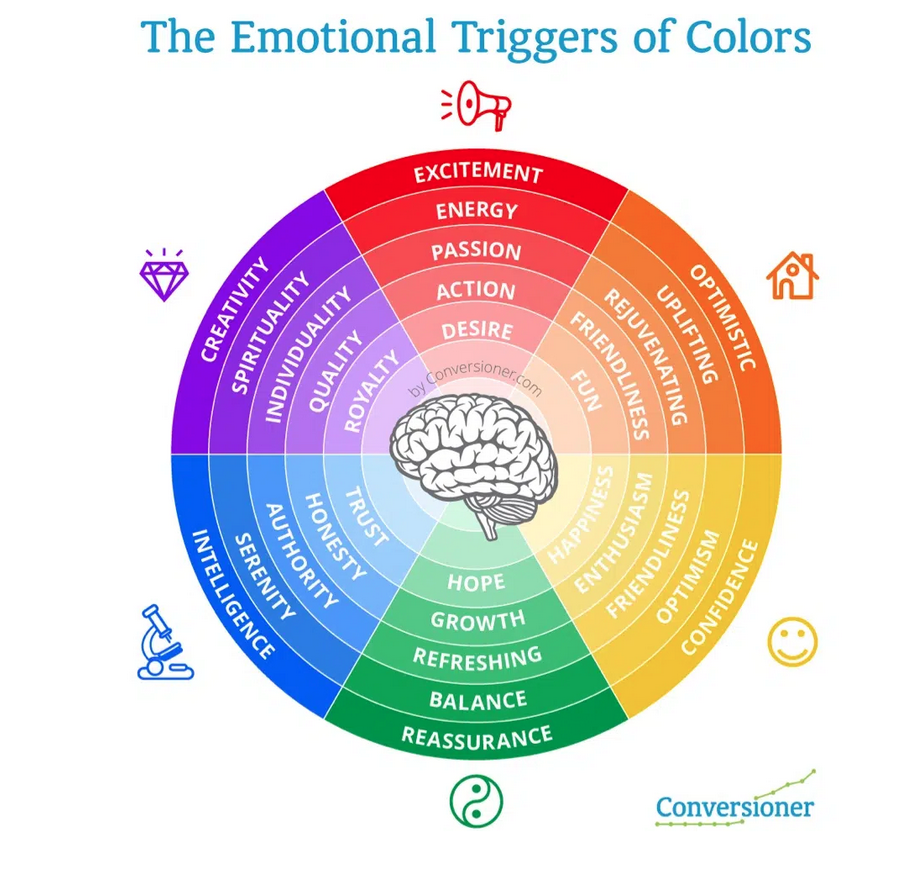
\includegraphics[width=0.8\textwidth]{bilder/farbkreis.png}
\caption{Ein aktueller Farbkreis \cite{DesignEmo2003}}
\label{fig20:farbkreis}
\end{figure}\\

Die Wahl von geringen Kontrasten spielt ebenfalls eine wichtige Rolle bei der Schaffung einer gelassenheitserzeugenden Webseite. Hohe Kontraste können die Aufmerksamkeit des Benutzers stark beanspruchen und eine gewisse Unruhe verursachen. Indem man sich für geringere Kontraste entscheidet, schafft man eine harmonische und ausgewogene visuelle Erfahrung. Die Augen des Nutzers werden nicht durch starke Unterschiede zwischen den Farben belastet, sondern können sanft über die Webseite gleiten, was zu einem entspannten und angenehmen Surferlebnis führt.\\
Ein Kontrast von 6.37:1 ist niedrig. \\

% Contrastchecker
\begin{figure}[H]
    \centering
    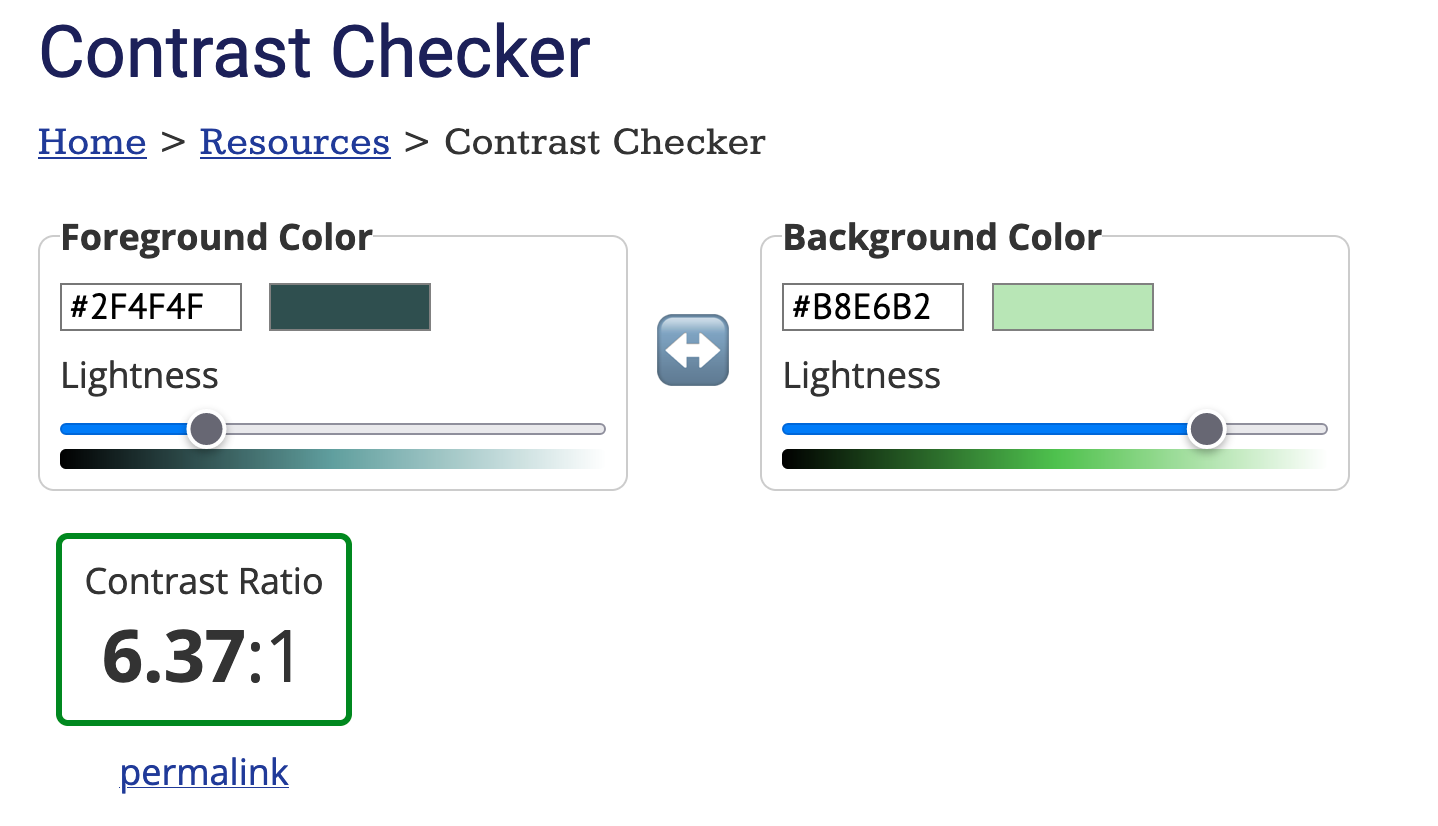
\includegraphics[width=0.8\textwidth]{bilder/contrast-gelassenheit.png}
    \caption{Das Kontrastverhältnis Schrift zu Hintergrund in dieser Anwendung}
    \label{fig21:contrast}
\end{figure}\\

\begin{figure}[H]
    \centering
    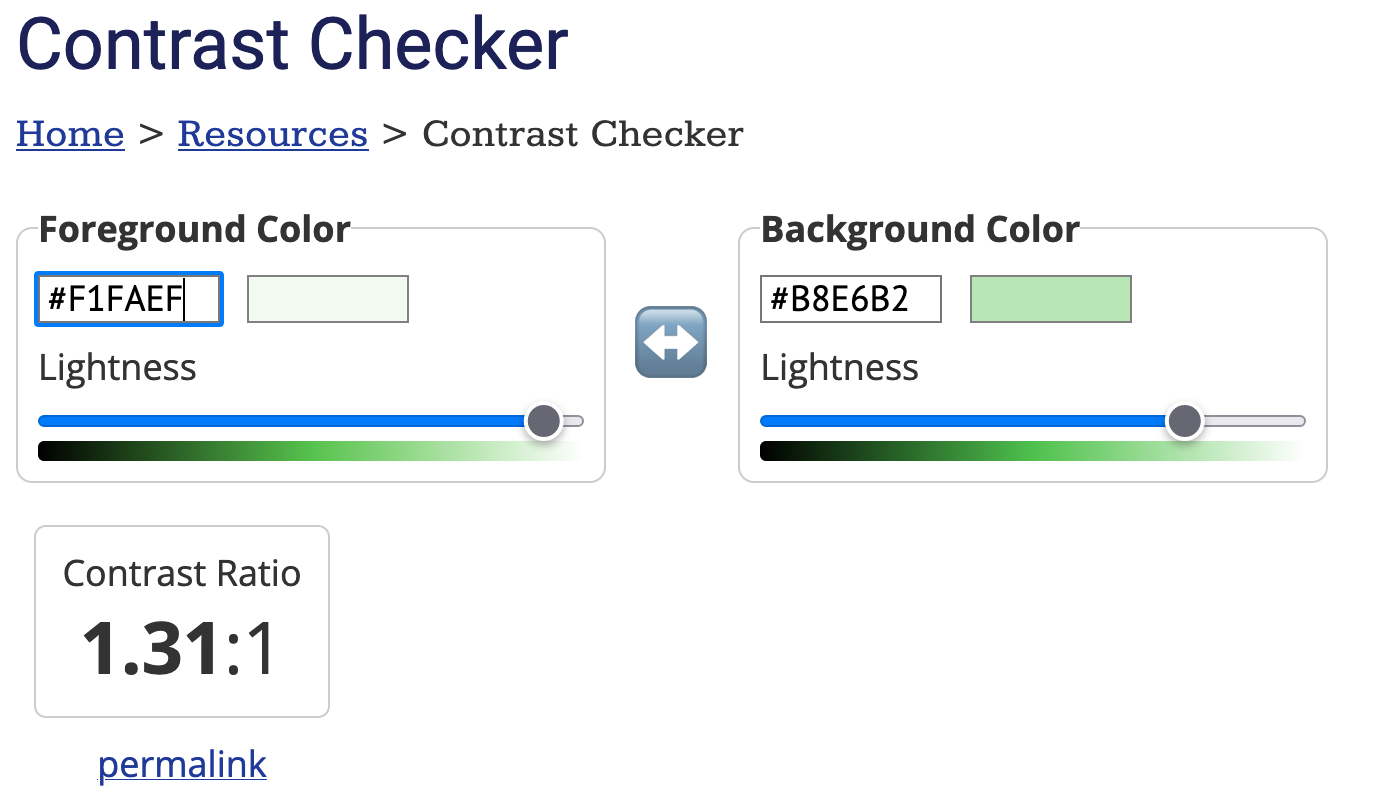
\includegraphics[width=0.8\textwidth]{bilder/contrast-box.png}
    \caption{Das Kontrastverhältnis Schrift zu Textbox in dieser Anwendung}
    \label{fig23:contrast}
\end{figure}\\

Des Weiteren ist die Reduktion ablenkender Elemente von großer Bedeutung, wenn es um die Erzeugung von Gelassenheit auf einer Webseite geht. Eine überladene und unübersichtliche Gestaltung kann den Nutzer überfordern und Stress verursachen. Durch die Reduktion von unnötigen visuellen Reizen kann der Fokus des Benutzers auf die wesentlichen Inhalte gelenkt werden. Dies fördert eine meditative Erfahrung und ermöglicht es dem Nutzer, sich auf das Wesentliche zu konzentrieren, ohne sich von irrelevanten Elementen ablenken zu lassen.\\

Die Kombination aus sanften Grüntönen, geringen Kontrasten und einer auf das Wesentliche reduzierten Gestaltung schafft also eine Webseite, die Gelassenheit und Entspannung fördert. Dies ist besonders relevant in einer Zeit, in der digitale Medien häufig mit stressigen und überwältigenden Erfahrungen in Verbindung gebracht werden. Eine gelassenheitserzeugende Webseite kann somit nicht nur das Wohlbefinden der Nutzer steigern, sondern auch eine positive Wahrnehmung und Bindung an die Webseite fördern.\\

% Farbpalette Adobe Color

\begin{figure}[H]
    \centering
    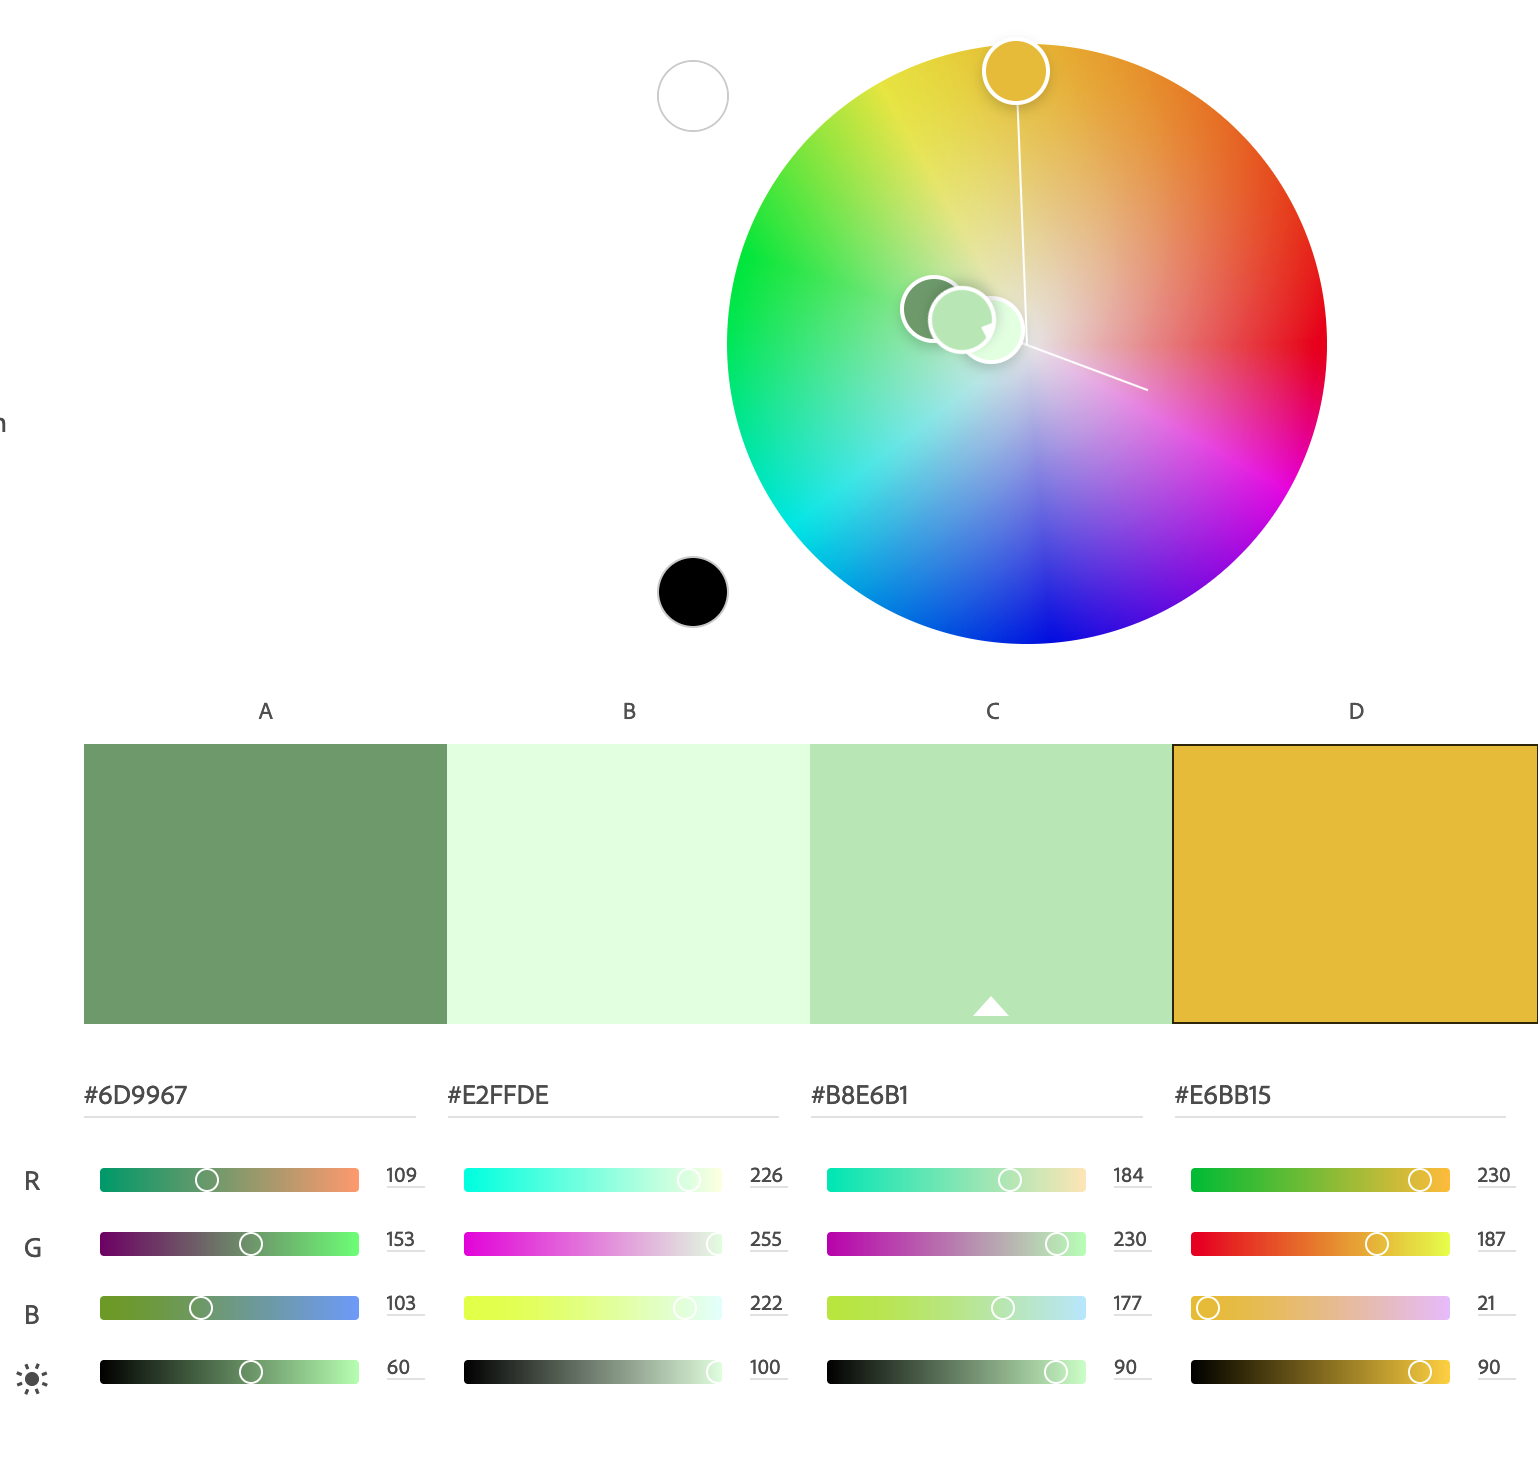
\includegraphics[width=0.8\textwidth]{bilder/adobecolor.png}
    \caption{Die gewählte Farbgestaltung}
    \label{fig22:adobecolor}
\end{figure}\\

Darüber hinaus wird durch Einhaltung des Gesetzes der Nähe eine leichte Orientierung ermöglicht.  Zusammenfassend lässt sich sagen, dass die bewusste Gestaltung von Webseiten durch die Wahl bestimmter Farben und Kontraste eine signifikante Auswirkung auf die emotionalen Zustände der Nutzer hat. Die gezielte Nutzung von sanften Grüntönen, geringen Kontrasten und einer reduzierten Gestaltung kann eine Atmosphäre der Gelassenheit schaffen und den Nutzern eine angenehme und entspannende Erfahrung bieten. Webseiten, die diese Gestaltungsprinzipien berücksichtigen, haben das Potenzial, eine nachhaltige und positive Wirkung auf das emotionale Wohlbefinden ihrer Besucher zu entfalten.\\

\begin{figure}[H]
    \centering
    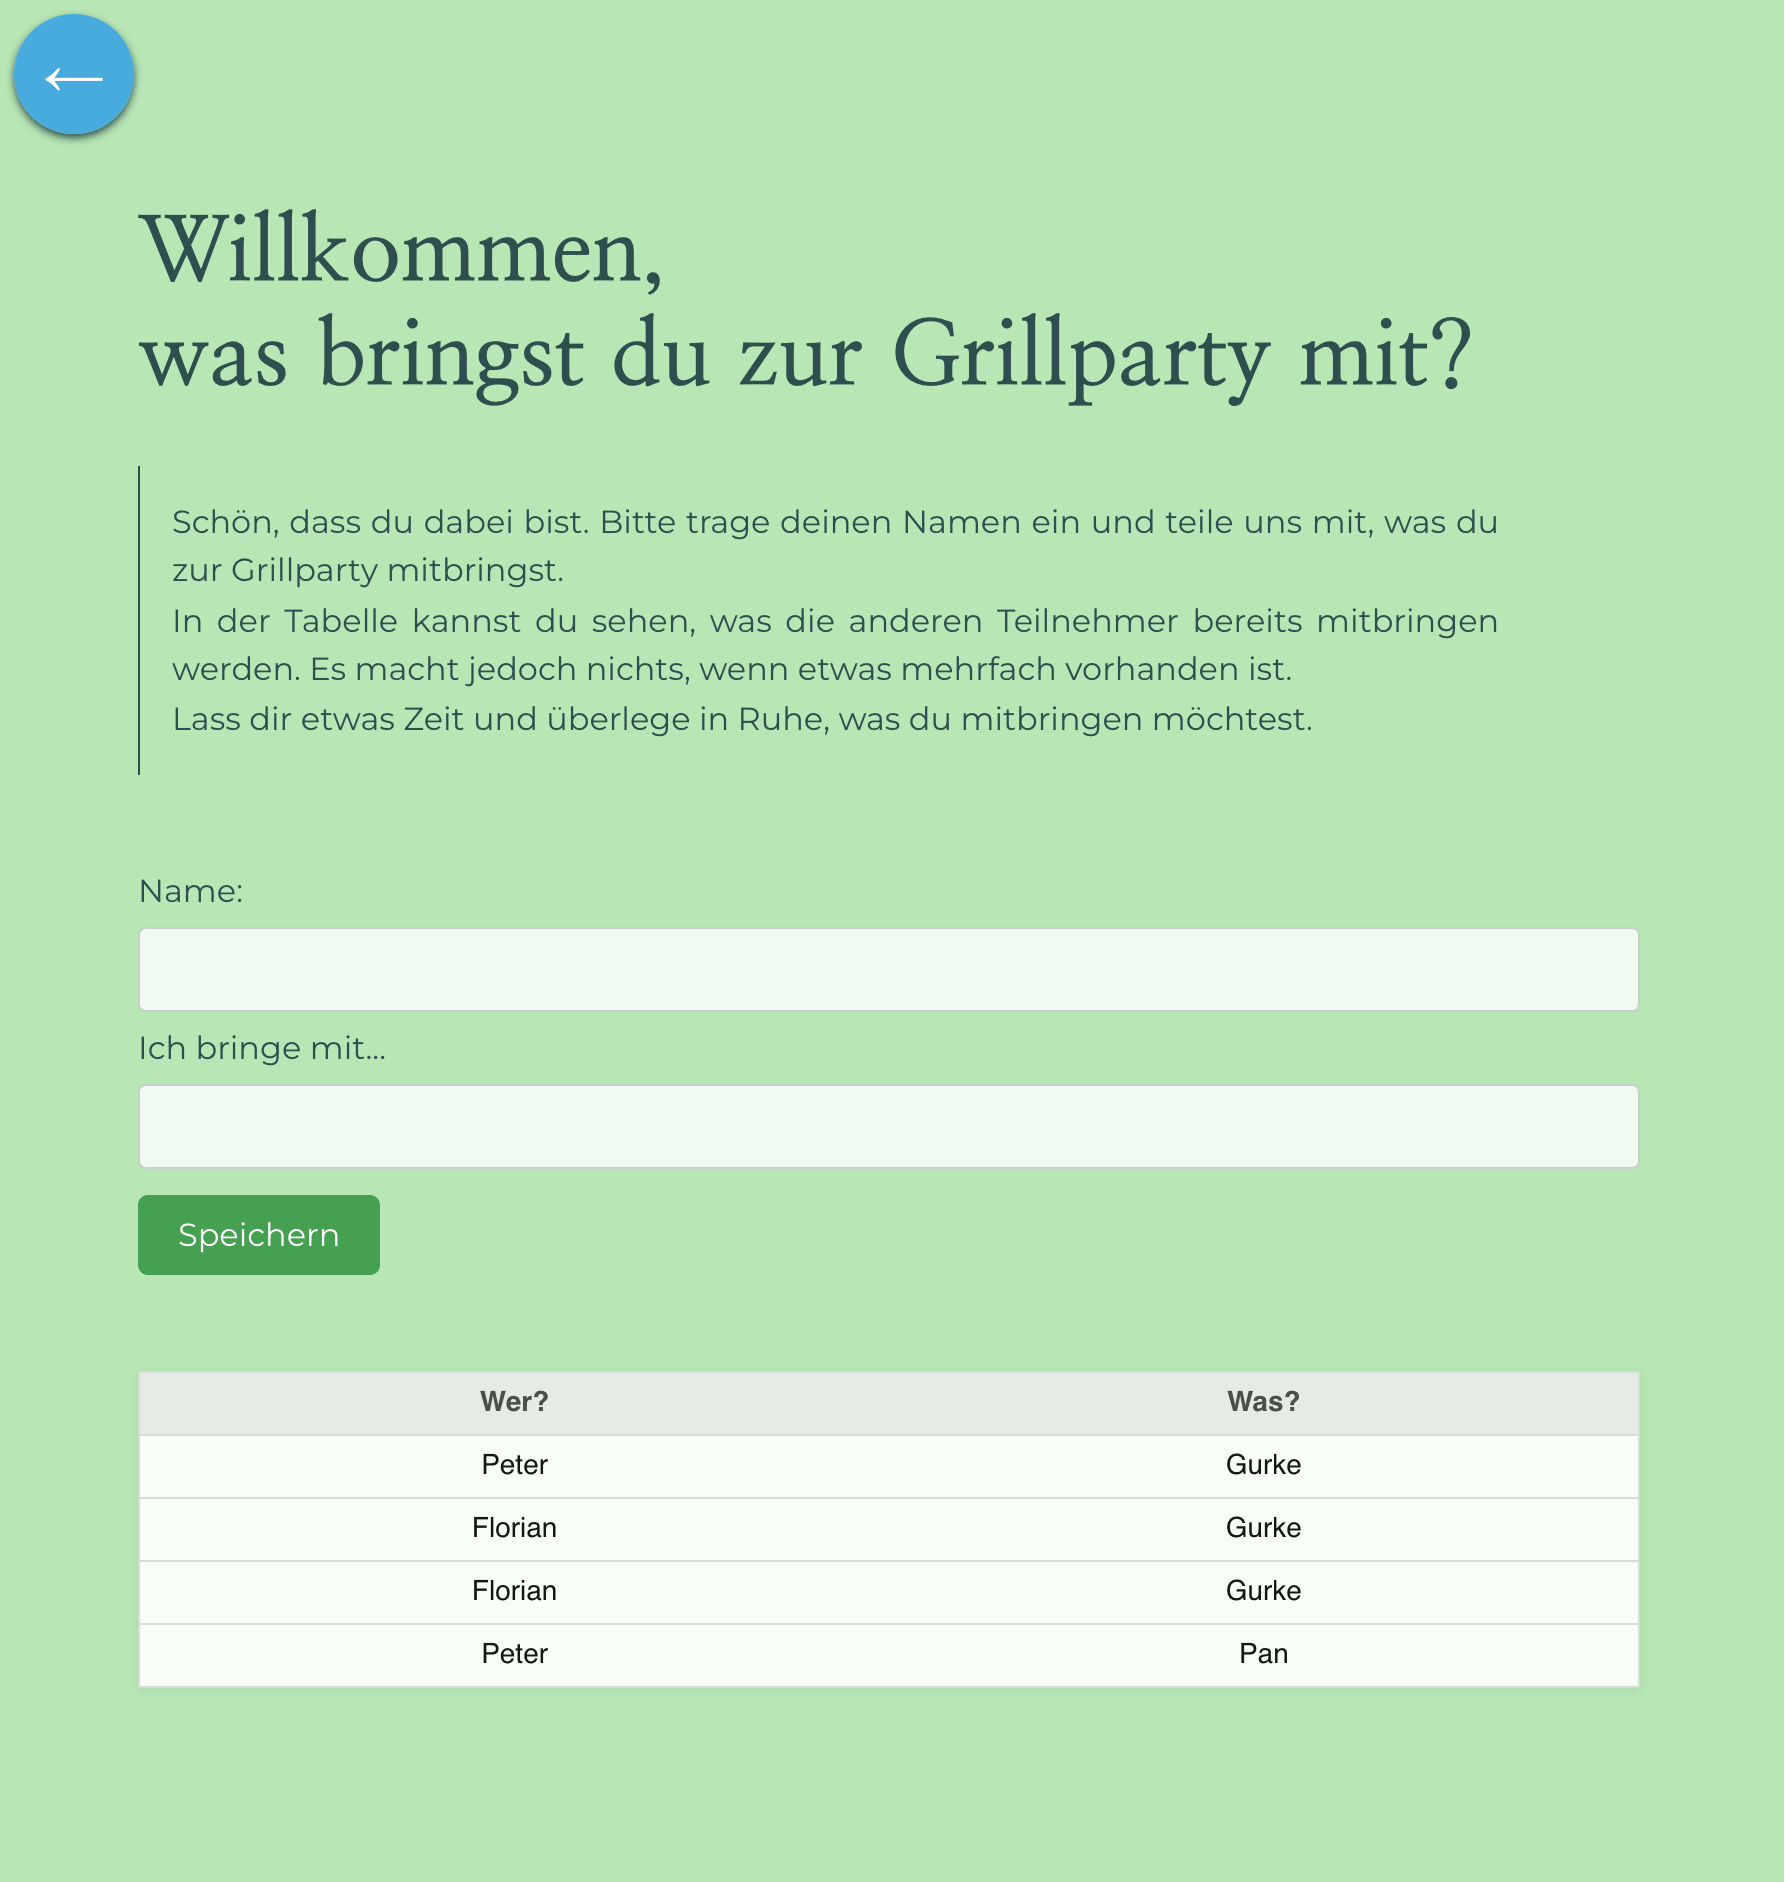
\includegraphics[width=0.8\textwidth]{bilder/website-gelassen.png}
    \caption{Die vollständige Website}
    \label{fig21:website-gelassen}
    \end{figure}\\

\begin{figure}[H]
        \centering
        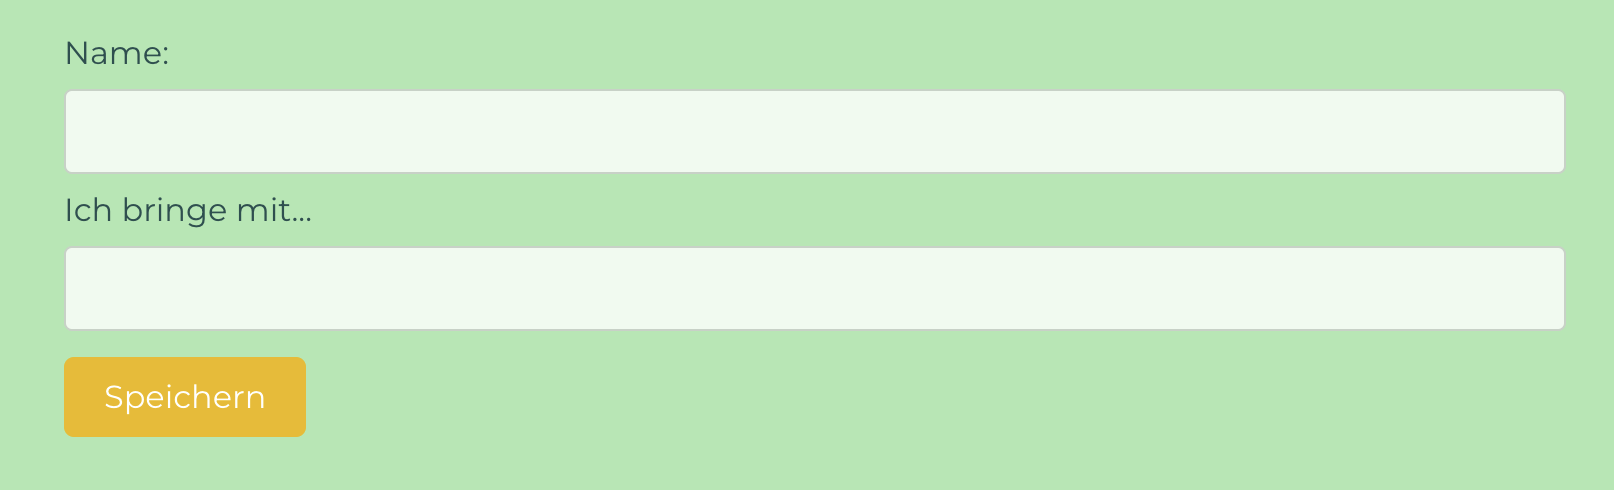
\includegraphics[width=0.8\textwidth]{bilder/website-gelassen-hover.png}
        \caption{Der Button wird bei Mouseover gelb}
        \label{fig22:website-gelassen-hover}
\end{figure}\\
    

\pagebreak
\section{Webseite - bewusstes Einsetzen der Elemente für die Induzierung von Nostalgie}
%% TODO


\pagebreak
\section{Webseite - bewusstes Einsetzen von negativen Emotionen Stress - Unsicherheit - Angst}
Im folgenden Teilprojekt wurden bewusst eher negative Emotionen eingesetzt. Wie in Kapitel X beschrieben bürgen diese jedoch oftmals auch ein sehr hohes Motivationspotenzial, wodurch der Nutzer eher geneigt sein kann, eine Handlung auszuführen.\\
Auch Dominanz spielt dabei eine wichtige Rolle, wie in Kapitel X beschrieben, führt diese typischerweise eher zu hoher Erregung und zu hoher Motivation. Dies wird durch folgende Gestaltung erreicht:\\
Harte Kanten, eckige Formen. Dies zeigt sich in den verwendeten Input-Feldern und dem eckigen Button. Auch die Schriftart ist sehr klar gehalten. Zusätzlich dazu wurden sehr harte Kontraste gewählt, die Trennung zwischen dem Schwarzen Hintergrund und den weißen Texten und Inputfeldern ist sehr stark.

\begin{figure}[H]
    \centering
    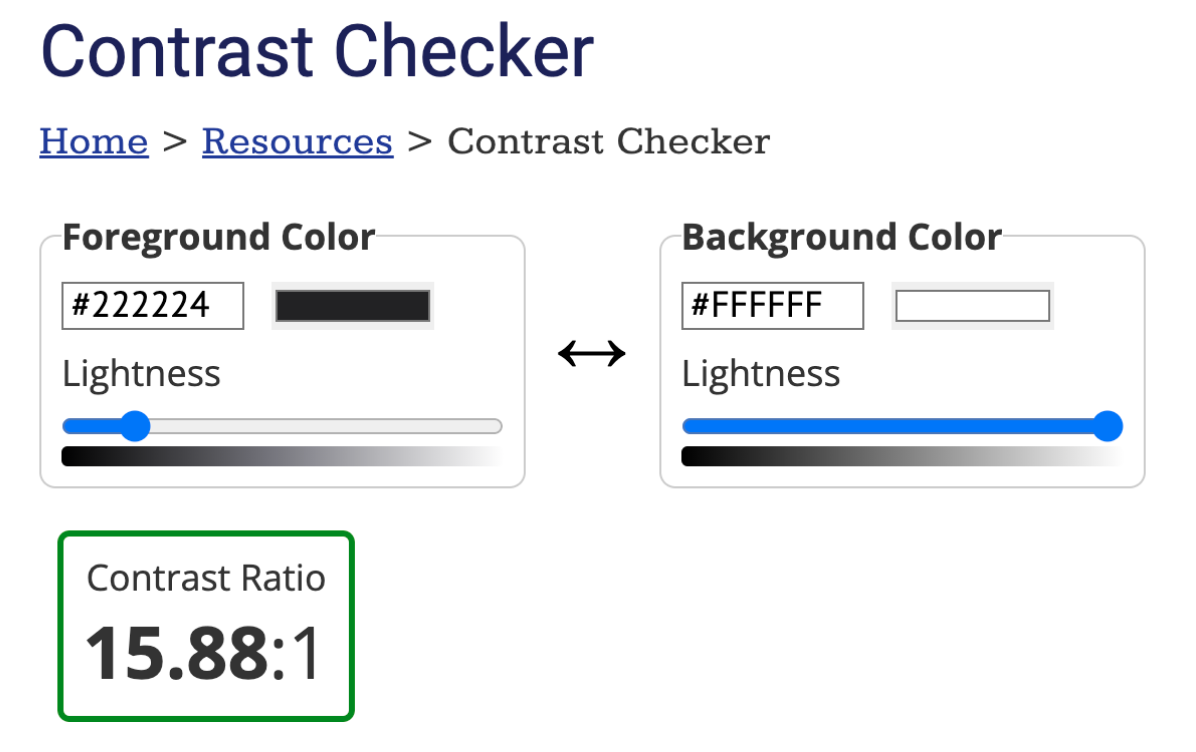
\includegraphics[width=0.8\textwidth]{bilder/contrast.png}
    \caption{Starke Kontraste} % TODO
    \label{fig12:contrast}
\end{figure}\\

\begin{figure}[H]
    \centering
    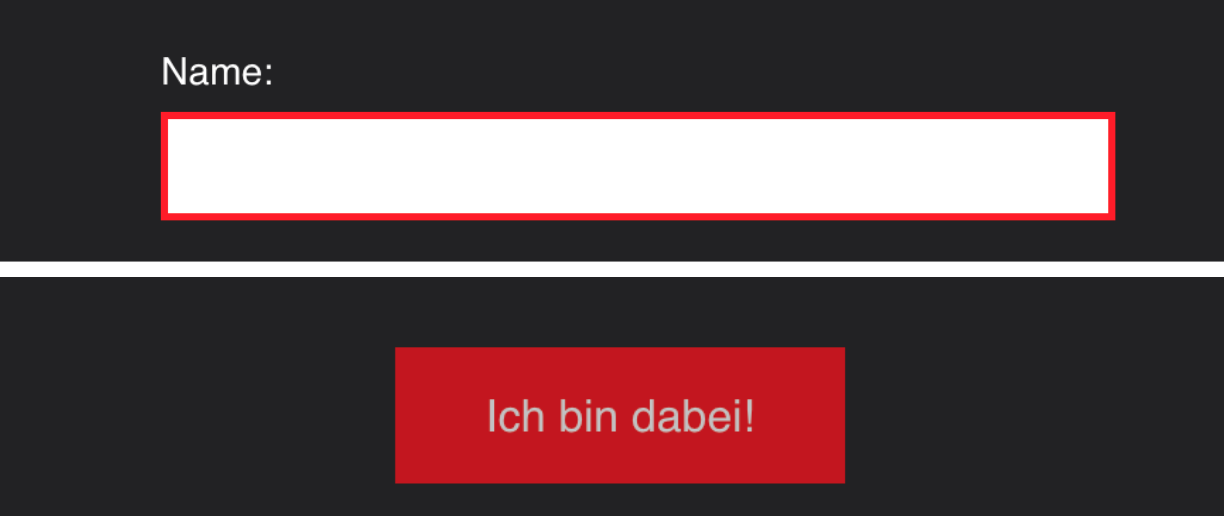
\includegraphics[width=0.8\textwidth]{bilder/name-bin-dabei.png}
    \caption{Eintragen des Namens und Submit-Button} % TODO
    \label{fig13:name}
\end{figure}\\

\subsection{Stress}
Um den Nutzer unter Druck zu setzen und ein Handeln zu forcieren, wurden hauptsächlich Blink-Effekte eingesetzt. Zusätzlich dazu wurde auch durch Storytelling, mit dem Hinweis, dass nur noch wenige Plätze verfügbar sind, Druck auf den Nutzer aufgebaut. Durch den Timer wird er weiter Stress ausgesetzt, der Druck wird durch das schrittweise Vergrößern der Schriftgröße zusätzlich unterstützt.\\
Im folgenden Screenshot sieht man den rot blinkenden Text, der darauf aufmerksam macht, dass nur noch 3 Plätze frei sind. Somit soll ein schnelles handeln erzwungen werden, bevor womöglich alle Plätze vergeben sind. Die rote Farbe als Signalfarbe deutet zusätzlich darauf hin, dass hier erhöhte Aufmerksamkeit gefordert ist.\\


\begin{figure}[H]
    \centering
    \includegraphics[width=0.8\textwidth]{bilder/schrift-freie-plätze3.png}
    \caption{Herabzählen der Anzeige erzeugt Stress}
    \label{fig14:platz}
\end{figure}\\


Mit Ablaufen des Timers vergrößert sich auch die Schrift. Dadurch wird noch mehr Aufmerksamkeit erzwungen und der Nutzer weiter unter Druck gesetzt.\\
Der Text zählt zunächst weiter runter und endet dann bei einem blinkenden “nur noch EIN Platz frei”, was suggeriert, dass nun endgültig gehandelt werden muss, bevor alle Plätze vergeben sind. Dies wird zusätzlich dadurch unterstützt, dass nun auch alle Input-Felder mit einem roten blinkenden Rahmen ausgestattet werden, sollten sie noch nicht ausgefüllt worden sein. \\


\begin{figure}[H]
    \centering
    \includegraphics[width=0.8\textwidth]{bilder/schrift-freie-plätze1.png}
    \caption{Herabzählen der Anzeige erzeugt Stress}
    \label{fig14:platz1}
\end{figure}\\

Auch der submit-button übernimmt den leuchtend roten, blinkenden Stil, wenn die Inputfelder erfolgreich ausgefüllt wurden und setzt den Nutzer unter Stress, um ein Handeln zu erzwingen.

% Bild button

\begin{figure}[H]
    \centering
    
\includegraphics[width=0.8\textwidth]{bilder/rot-dabei.png}
    \caption{Rot leuchtender Submit-Button}
    \label{fig15:submit}
\end{figure}\\


\subsection{Unsicherheit}

\begin{figure}[H]
    \centering
    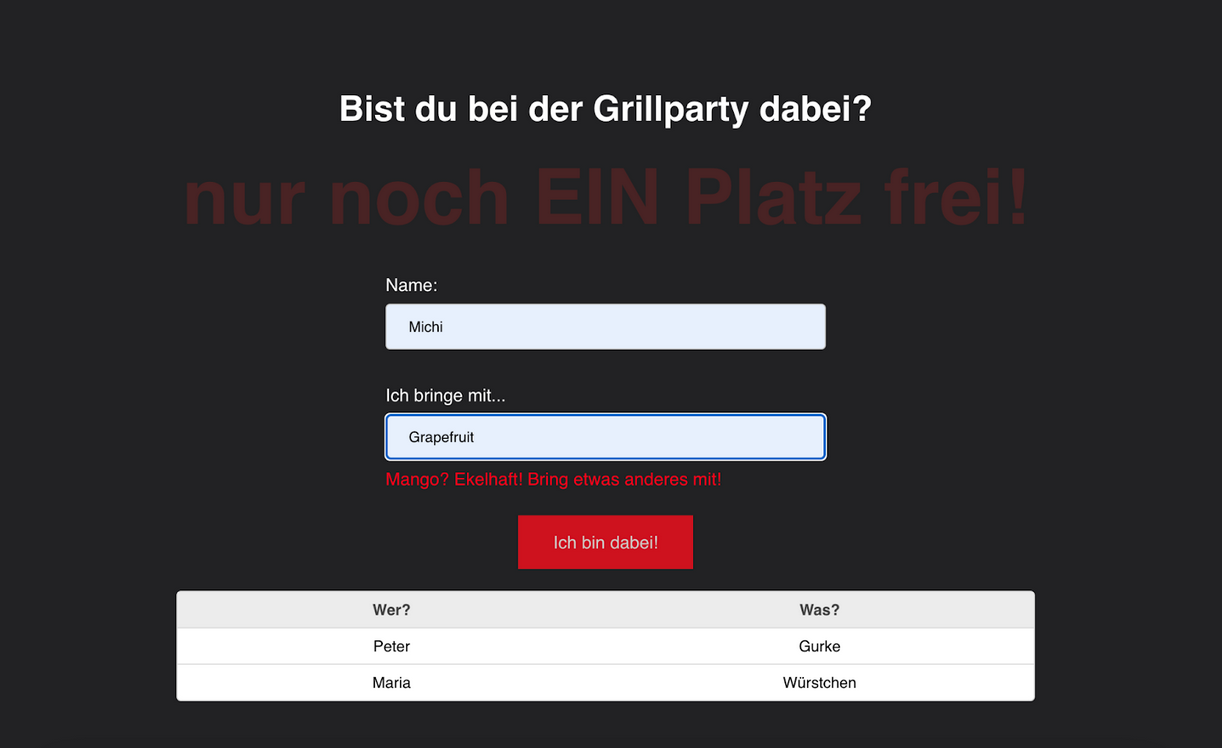
\includegraphics[width=0.8\textwidth]{bilder/ekelhaft.png}
    \caption{Unfreundliche Kommunikation} %% TODO
    \label{fig16:ekel}
\end{figure}\\


\begin{figure}[H]
    \centering
    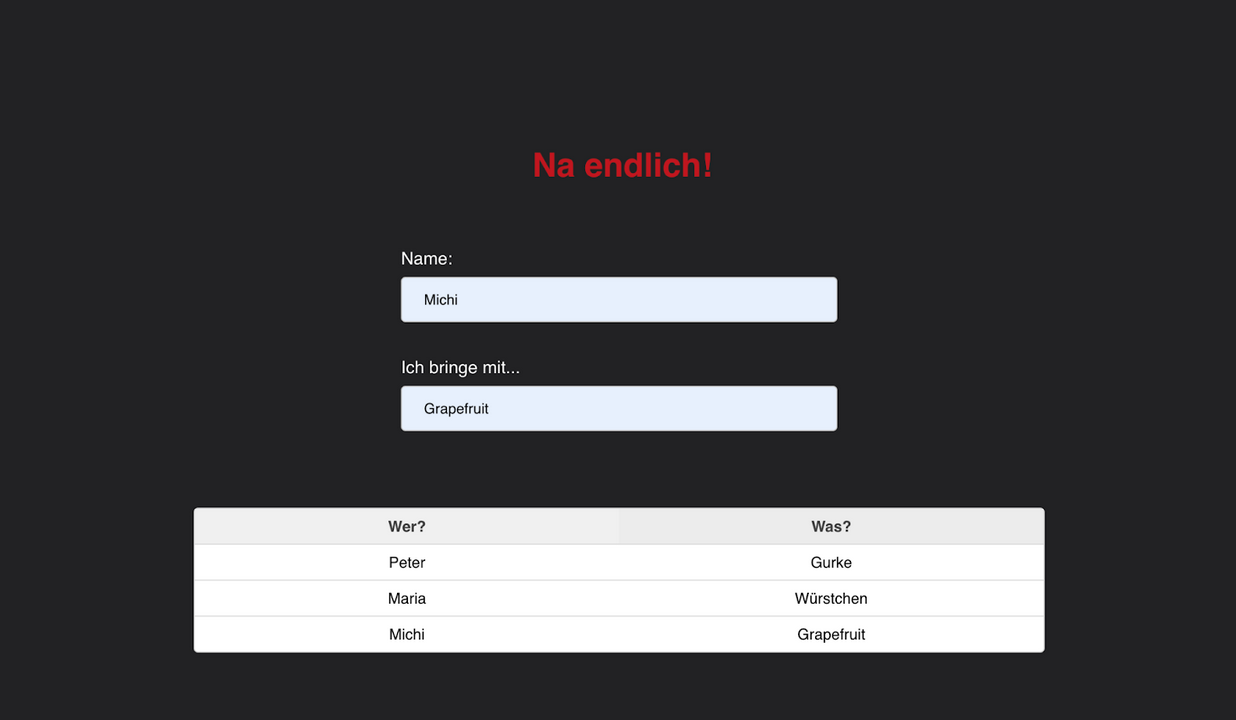
\includegraphics[width=0.8\textwidth]{bilder/na-endlich.png}
    \caption{Letztlich wird die Eintragung vorgenommen}
    \label{fig17:okay}
\end{figure}\\


\subsection{Angst}
Auch Angst als sehr starke Emotion  kann genutzt werden, um Handlungen zu forcieren. Hierbei muss man auch aufpassen, dass diese nicht zu stark ist, sodass der Nutzer noch handlungsfähig ist. Wird Angst richtig dosiert, kann sie dazu beitragen, dass sich Botschaften beim Nutzer besser einprägen. Im Beispiel der hier betrachteten Webseite wird diese durch die dunklen Farben unterstützt und die Darstellung des angstvollen/aufmerksamen Gesichts (insbesondere Augenpartie), das sehr groß auf der Webseite dargestellt ist und zusätzlich durch die Animation der Augen Aufmerksamkeit generiert. Somit soll der Nutzer animiert werden, auch wirklich zu der Grillparty zu kommen.\\

\begin{figure}[H]
    \centering
    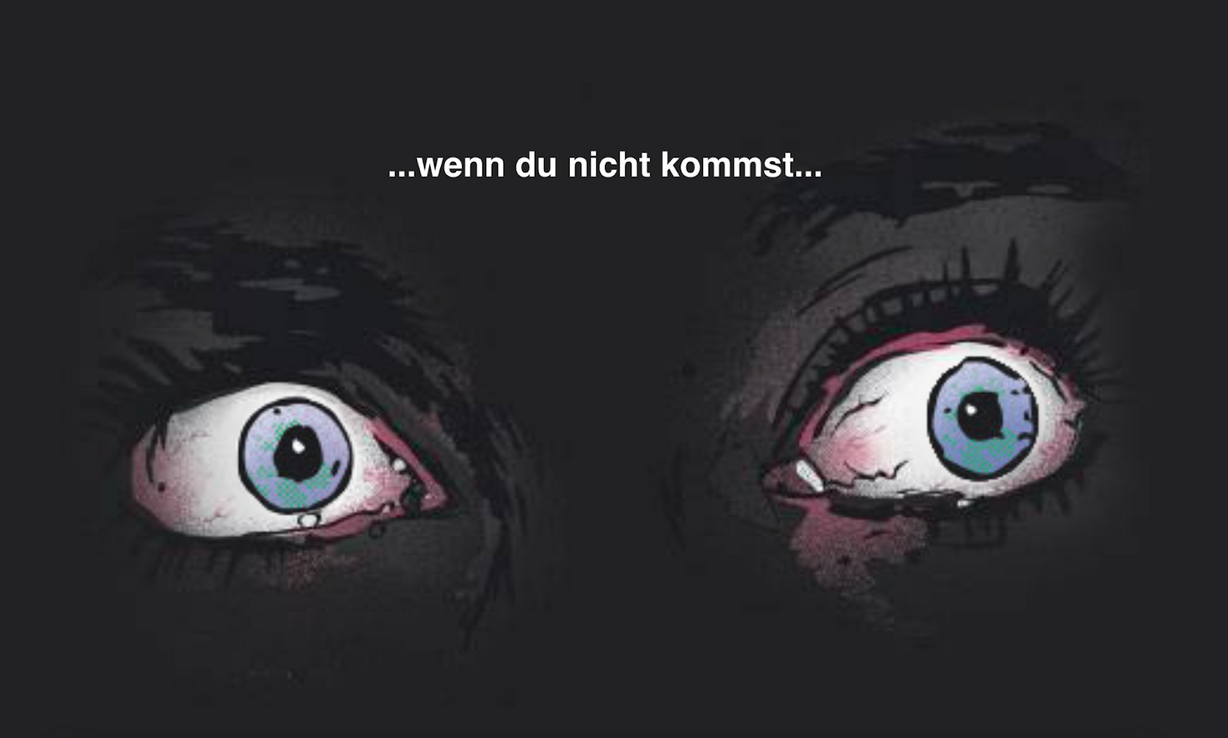
\includegraphics[width=0.8\textwidth]{bilder/angst1.png}
    \caption{Bewusstes erzeugen von Angst}
    \label{fig18:angst1}
\end{figure}\\

\begin{figure}[H]
    \centering
    
\includegraphics[width=0.8\textwidth]{bilder/angst2.png}
    \caption{Bewusstes erzeugen von Angst}
    \label{fig19:angst2}
\end{figure}\\

\section{Implikationen}
\subsection{Sprachliche Relativität}
In Anbetracht der Gestaltung der Website, ist die Sapir-Whorf-These zu benennen. Laut dieser These kann die Art und Weise, wie wir denken, durch die semantische Struktur unserer Sprache divergieren \cite{Cibelli2016}. Eine Abgeleitete Hypothese von Roberson et. al (2006) hat dafür weitere Hinweise festgestellt. So soll ein indigener Stamm aus Namibia mit dem Test aus Abbildung X konfrontiert worden sein. Die Zielgruppe wurde dazu aufgefordert das Quadrat zu finden, das nicht die gleiche Farbe hat wie der Rest. Bei dem ersten Test wurden alle Farben als gleich betitelt, es konnte kein andersfarbiges Quadrat festgestellt werden. Bei dem zweiten Test hingegen wurde ein Unterschied festgestellt. Beachtlich ist dies, da der Kontrast aus dem ersten Test verglichen mit dem des 2. Test deutlich erkennbar  ist, für Individuen unseres Kulturkreises.\\
In dieser Arbeit wir also die emotionale Wirksamkeit bestimmter Gestaltungselemente unseren Kulturkreises berücksichtigt und ist somit nicht anwendbar auf die gesamte Bevölkerung. 


\end{document}


